\providecommand{\mainpath}{..} % Command to retrieve the path of the main file. It must be defined before documentclass.

\documentclass[\mainpath/main]{subfiles}
\begin{document}

\chapter{Project Estimations} % First chapter
\label{ProjectEstimation}

% Command to be executed after the starting of every chapter
\setmyfancystyle
% ----------------

In this chapter we are going to estimate the main features of \textit{myTaxiService} project, by using COCOMO II. Reading from the reference manual:
\begin{quote}
	\textit{The COCOMO II model is part of a suite of Constructive Cost Models. This suite is an effort to update and extend the well-known COCOMO (Constructive Cost Model) software cost estimation model originally published in Software Engineering Economics by Barry Boehm in 1981.}
\end{quote}
In the \autoref{ProjectEstimation:ProjectSize} we focus on the project's size in term of lines of code, whereas in the \autoref{ProjectEstimation:EffortEstimation} other metrics, such the required time and the costs will be analysed.



\section{Project Size (Function Points)}
\label{ProjectEstimation:ProjectSize}
Reading from the reference manual:
\begin{quote}
	\textit{The function point cost estimation approach is based on the amount of functionality in a software project and a set of individual project factors [Behrens 1983; Kunkler 1985; IFPUG 1994]. Function points are useful estimators since they are based on information that is available early in the project life-cycle. A brief summary of function points and their calculation in support of COCOMO II follows.}
\end{quote}
The function types are five, described in the table\footnote{The table is given by the COCOMO II reference manual.}.\\[0.2cm]
\begin{tabular}[!ht]{l@{\hspace{1cm}}p{8.5cm}}
	\hline  \textbf{Function Point} & \textbf{Description}\\ 
	\hline External Input (EI) & Count each unique user data or user control input type that enters the external boundary of the software system being measured.\\ 
	\hline External Output (EO) & Count each unique user data or control output type that leaves the external boundary of the software system being measured.\\ 
	\hline Internal Logical File (ILF) & Count each major logical group of user data or control information in the software system as a logical internal file type. Include each logical file (e.g., each logical group of data) that is generated, used, or maintained by the software system.\\
	\hline External Interface Files (EIF) & Files passed or shared between software systems should be counted as external interface file types within each system.\\
	\hline External Inquiry (EQ) & Count each unique input-output combination, where input causes and generates an immediate output, as an external inquiry type.\\ \hline \\[1cm]
\end{tabular}

Finally, to perform the analysis we have to present other two tables from the same reference manual of the other one. The first one will be used to classify each function on three level of complexity (high, medium and low).

\begin{figure} [!ht]
	\centering
	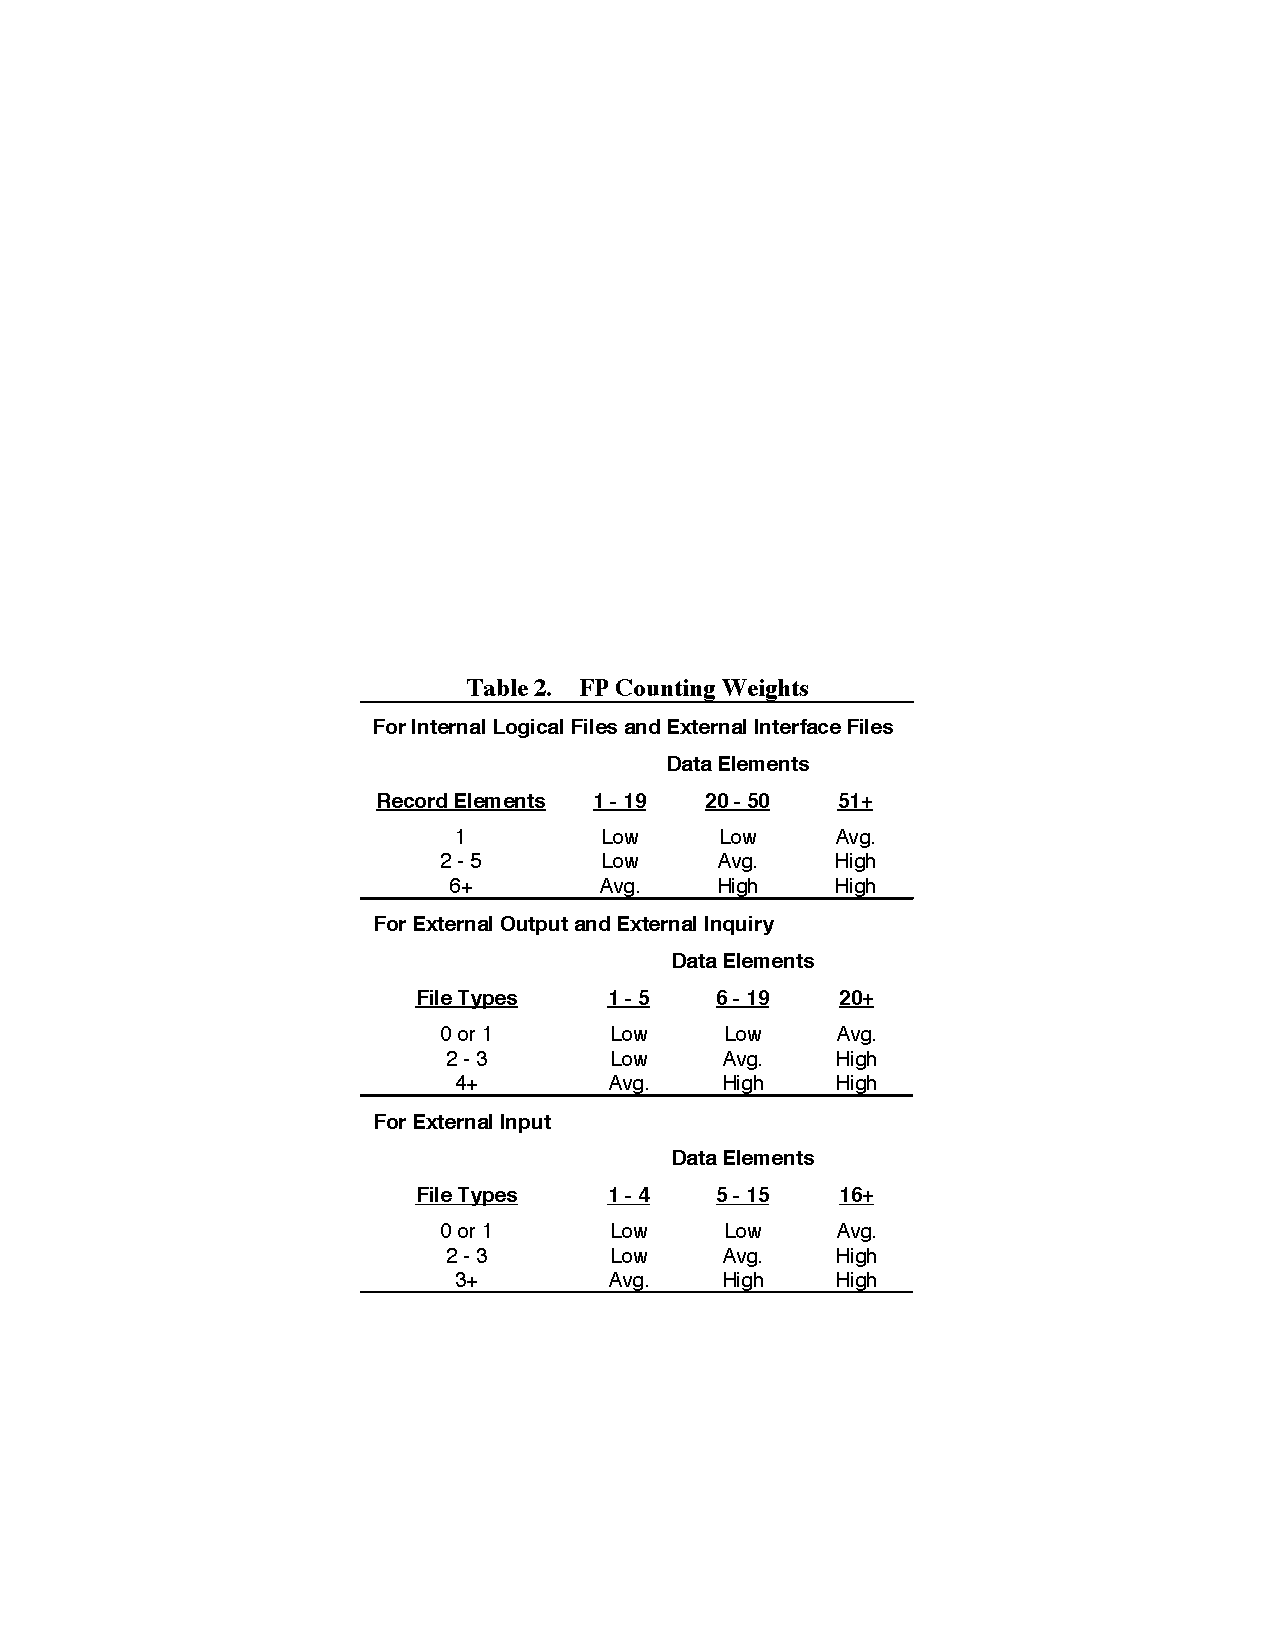
\includegraphics{table/complexity}
\end{figure}

The second one shows the weights to be used into the estimation formulas\footnote{The UFP acronym means Unadjusted Function Points}.

\begin{figure}[!ht]
	\centering
	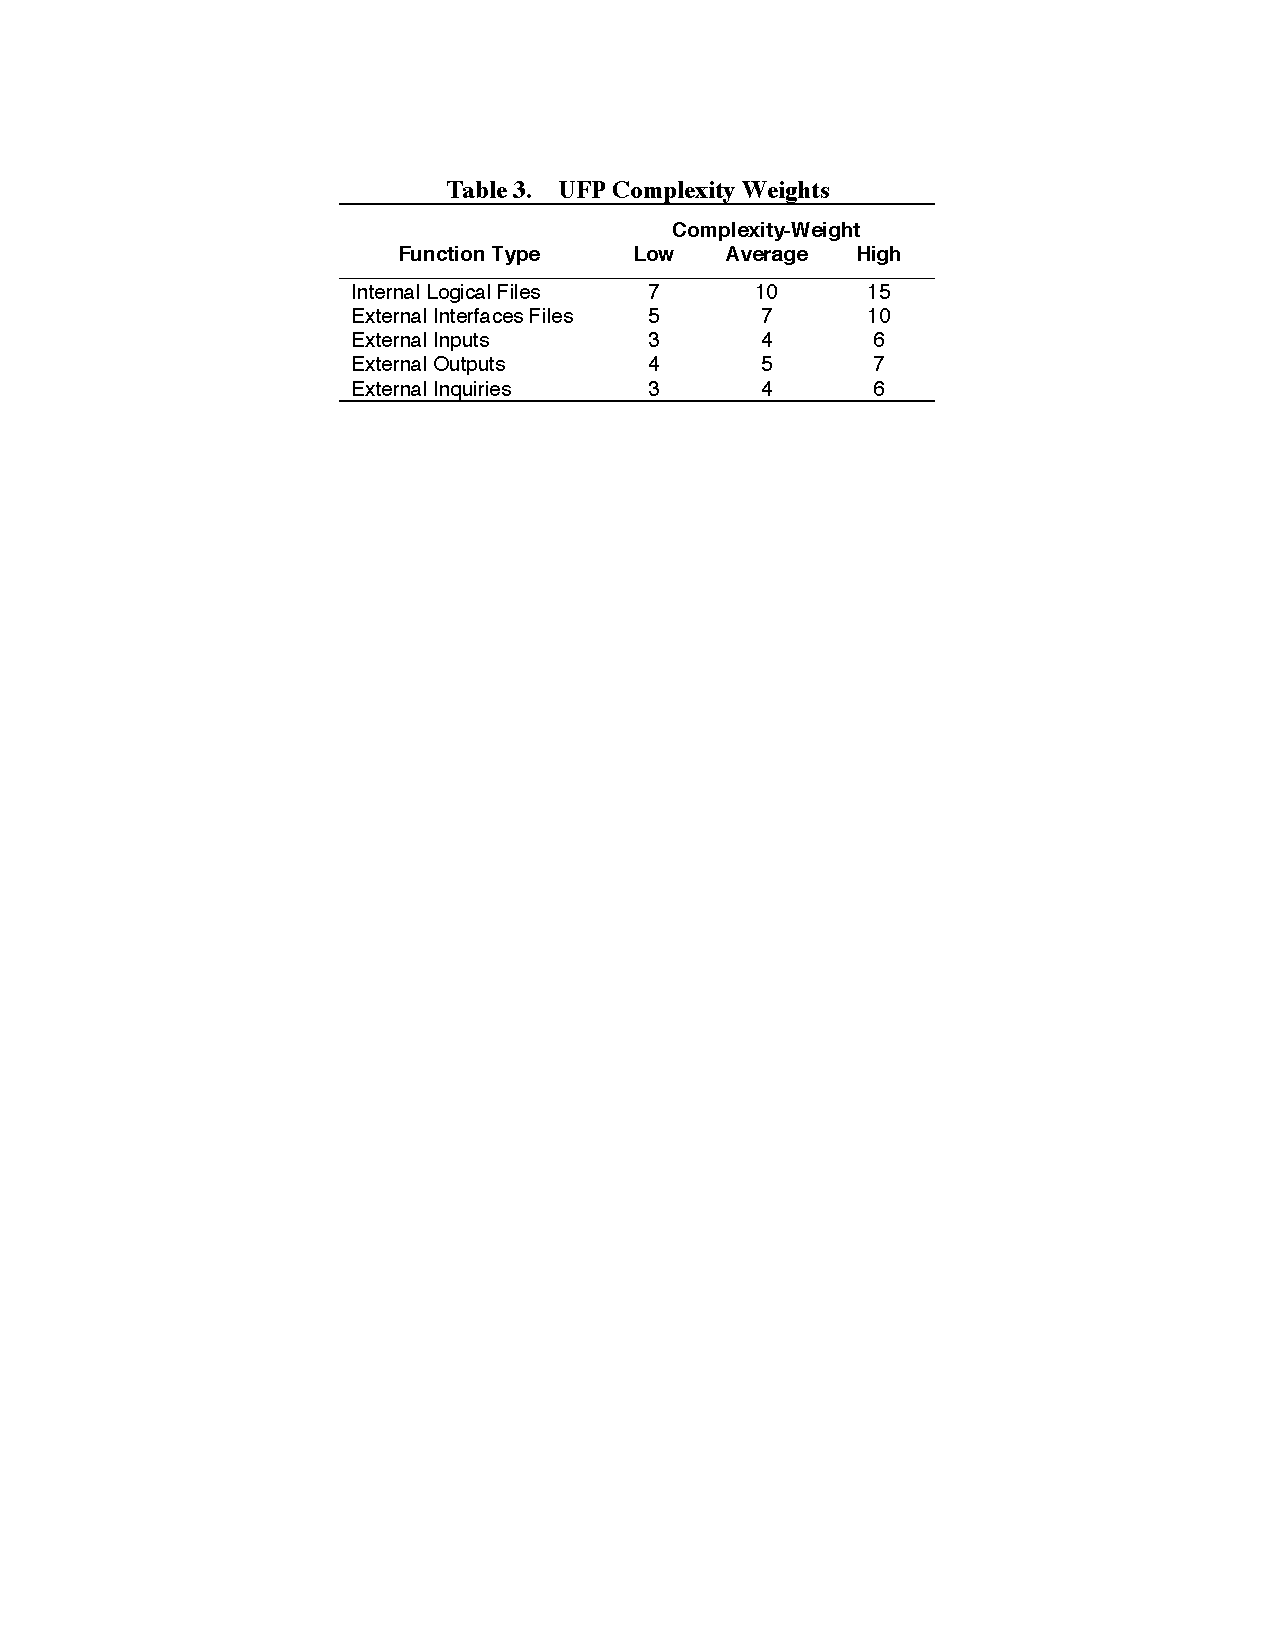
\includegraphics{table/weights}
\end{figure}

\clearpage

Up to now, we have presented the Function Points technique. Now, we are going to start our analysis, split by the function type.

\subsection{Internal Logic Files}
The system has to manage Internal Logic Files to store information related to the users (both \textit{normal} and drivers), the \textit{historical} rides, the areas and the driver work shifts\footnote{See the logic schema at the page 10 of the Design Document to have a detailed description of each part of the database.}\\
The users have from 12 to 16 fields to be stored (the second number is referred to the drivers case) and only the alerts and the zerotime or future rides have to be stored, thus the complexity is low. The areas and the work shifts can also be considered as low complexity type. In fact they have a few fields and less than six extra records.\\
The rides have 10 fields, including two positions, the driver and the passenger, all saved in separate entities. They can be considered as an average complexity type, since we have about seven records per ride (in fact in addition to the five presented, the positions requires additional records).\\
In the table the analysis is summarize:
\begin{tabular}{ccc}
	\hline ILF & Complexity & FP \\
	\hline User & Low & 7 \\
				Area & Low & 7 \\
				Workshift & Low & 7 \\
				Ride & Average & 10 \\
	\hline Total & & 31
\end{tabular}

\subsection{External Logic Files}
The system acquires data from te GPS interface. A GPS position is essentially a tuple of type Position, described in our database. Hence, we have a low complexity type and 5 FP.

\subsection{External Inputs}
The possible interactions between the users and the system, defined in the RASD, are now quickly described in terms of complexity:
\begin{itemize}
	\item Login/Logout: these operations are simple due to one entity only is involved, so the complexity is low;
	\item Start Waiting Time/End of a ride: these operation requires to interact with three types of files (Position, Area and Driver Waiting) with one element per type, thus the complexity is low;
	\item Check the Reservations: this is a group of three related operations (shows the alerts and gives the possibilities to modify or to cancel a ride) that involve one type and potentially more than 16 elements, so the complexity is average;
\end{itemize}
In the following table we have summarized the results:\\[0.5cm]
\begin{tabular}{p{7cm}@{\hspace{1.5cm}}p{5cm}r}
	\hline EI & Complexity & FP \\
	\hline Login/Logout & Low & 2x3 \\
	Start Waiting Time / End of a Ride & Low & 2x3 \\
	Check the Reservations & Average & 3x4 \\
	\hline Total & & 24
\end{tabular}

\subsection{External Inquiries}
The system allows the user to interact with it through the following operations:
\begin{itemize}
	\item Registration: this operation is performed only by simple user (not a driver) and involves one data type, the one related to the new user. Its complexity is low;
	\item Profile Management: this operation allows the user to modify a little personal data, so the complexity is low;
	\item Work shift Management: this operation requires to interact to 2 entities (driver and work shift) and can involve more than 20 elements to perform the validity checks. Hence the complexity is high;
	\item Book a ride (both future or zerotime): these operations needs many interactions between the system and the user, for instance to show the detected position or to analyse the inserted time/address;
	\item Ride Allocation: we also insert this function because the system has to interact in a simple way with the taxi driver. Since many and many taxi drivers or queues may be involved before one is available, the complexity is high. Note that the notifications of the operations are not reported here, but in the External Input section;
	\item Taxi Driver Ride Request: this is the operation used to ask a rider the availability for a ride, the complexity is low.
\end{itemize}
In the following table we have summarize the results:\\[0.5cm]
\begin{tabular}{p{7cm}@{\hspace{1.5cm}}p{5cm}r}
	\hline EQ & Complexity & FP \\
	\hline Registration & Low &  3\\
	Profile Management & Low & 3\\
	Workshift Management & High & 6\\
	Book a ride & High & 2x6\\
	Ride Allocation & High & 6 \\
	Taxi Driver Ride Request & Low & 3 \\
	\hline Total & & 33
\end{tabular}

\subsection{External Outputs}
The external outputs shown by the system are all related with the notifications. In fact the system administrators can notify all the users about service situations (for instance a strike, an incident that forbids the access in some city areas and so on). Other kind of notifications, are the ones about the requested ride's status.\\
Finally we have the operations of shown these notifications (Read the Alerts). All the described operations have to interact with about three types of record (always the user and the alert. If any, also other files are involved, as the ride or the position) and many files (both users or old alerts when we are showing the alerts), thus the complexity is high. Instead, the ride status notifications have to interact with one user, so the complexity is low.\\
The results are summarized in the following table:\\[0.2cm]
\begin{tabular}{l@{\hspace{1cm}}cc}
	\hline EO & Complexity & FP \\
	\hline System Notifications & High & 7\\
			   Ride Status Notifications & Low & 4\\
			   Read The Alerts & High & 7\\
	\hline Total & & 18\\
\end{tabular}

\subsection{Final Results}
The Function Point found in the previous sections are reported in the following table:\\[0.2cm]
\begin{tabular}{p{12cm}@{\hspace{1cm}}r}
	\hline Function Type & Value \\
	\hline Internal Logic Files (ILF) & 31\\
			   External Logic Files (ELF) & 5\\
			   External Inputs (EI) & 24\\
			   External Inquiries (EQ) & 33\\
			   External Outputs (EO) & 18\\
	\hline Total & 111\\[0.5cm]
\end{tabular}
	
Since our project has no a specific programming language to be used, in the following table we report the project size estimations both for the C++ and for the Java. In addition we report a few interesting measure with C, Assembler and Machine Code:\\[0.2cm]
\begin{tabular}{p{5.5cm}@{\hspace{1cm}} p{4cm}@{\hspace{1cm}} r}
	\hline Programming Language & UFP to SLOC Conversion Ratios\footnotemark & Lines of Code \\
	\hline Java & \centering 53 & 5833\\
			   C++ & \centering 55 & 6105\\
	\hline C & \centering 128 & 14208\\
			   Assembly - Basic & \centering 320 & 35520\\
			   Machine Code & \centering 640 & 71040 \\ \hline
\end{tabular}
\footnotetext{The values are still taken from the COCOMO II reference manual.}


\section{Effort Estimation (COCOMO II)}
\label{ProjectEstimation:EffortEstimation}
In this section we make an Effort Estimation using the model of COCOMO II. Following this model we can calculate the required effort measured in Person-Months with the effort equation, that is:
\begin{equation}
	effort = 2.94 * EAF * (KSLOC)^E
	\label{ProjectEstimation:effort-equation}
\end{equation}

where the first factor \textbf{$2.94$} is a constant calculated by COCOMO II 2000.0, \textbf{EAF} is the \textit{Effort Adjustment Factor} calculated as the product of the effort multipliers corresponding to each of the \textit{Cost Drivers}, \textbf{KSLOC} is the estimated number of lines of code calculated at the end of \autoref{ProjectEstimation:ProjectSize} and measured in thousands, the exponent \textbf{E} is the exponent derived from the \textit{Scale Drivers}.\\
\\
First we calculate the \textit{Scale Drivers} in the first subsection and then the \textit{Cost Drivers}. Finally we will compute the result of the effort equation presented above and also the duration of the necessary work to complete the project and the number of required people.

\subsection{Scale Drivers}
The exponent \textbf{E} in equation \ref{ProjectEstimation:effort-equation} is an aggregation of five scale factors (SF) that account
for the relative economies or diseconomies of scale encountered for software projects of different
sizes. These five scale factors with their corresponding numerical values are represented in the \autoref{ProjectEstimation:ScaleFactorTable}

\clearpage

\begin{table}
	\caption{Scale Factor Values, $SF_{j}$, for COCOMO II Models}
	\label{ProjectEstimation:ScaleFactorTable}
	\footnotesize
\begin{tabular}{|C{1.2cm}|C{1.8cm}|C{1.8cm}|C{1.8cm}|C{1.8cm}|C{1.8cm}|C{1.8cm}|}
	\hline \textbf{Scale Factors} & \textbf{Very Low} & \textbf{Low} & \textbf{Nominal} & \textbf{High} & \textbf{Very High} & \textbf{Extra High} \\ 
	\hline \textbf{PREC} & thoroughly unprecedented & largely unprecedented & somewhat unprecedented & generally familiar & largely familiar & thoroughly familiar \\ 
		   \textbf{SF$_{j}$} & 6.20 & 4.96 & 3.72 & 2.48 & 1.24 & 0.00 \\ 
	\hline \textbf{FLEX} & rigorous & occasional relaxation & some relaxation & general conformity & some conformity & general goals \\ 
		   \textbf{SF$_{j}$} & 5.07 & 4.05 & 3.04 & 2.03 & 1.01 & 0.00 \\
	\hline \textbf{RESL} & little (20\%) & some (40\%) & often (60\%) & generally (75\%) & mostly (90\%) & full (100\%) \\ 
		   \textbf{SF$_{j}$} & 7.07 & 5.65 & 4.24 & 2.83 & 1.41 & 0.00 \\ 
	\hline \textbf{TEAM} & very difficult interactions & some difficult interactions & basically cooperative interactions & largely cooperative & highly cooperative & seamless interactions \\ 
		   \textbf{SF$_{j}$} & 5.48 & 4.38 & 3.29 & 2.19 & 1.10 & 0.00 \\
	\hline \textbf{PMAT} & SW-CMM Level 1 Lower & SW-CMM Level 1 Upper & SW-CMM Level 2 & SW-CMM Level 3 & SW-CMM Level 4 & SW-CMM Level 5 \\ 
		   \textbf{SF$_{j}$} & 7.80 & 6.24 & 4.68 & 3.12 & 1.56 & 0.00 \\
	\hline 
\end{tabular} 
\end{table}

The scale factors and their values for our project are:

% TODO: Magari posso andare più nel dettaglio di ogni singolo scale factor

\begin{itemize}
	\item \textbf{PREC - Precedentedness:}\\
	Reflects the previous experience of the organisation with this type of project. Since we haven't realised before this kind of commercial, distributed and multi-platform system (accessible both via website and smartphone), the value of this scale factor is \textit{Low} (4.96).
	
	\item  \textbf{FLEX - Development Flexibility:}\\
	Reflects the degree of flexibility in the development process. The instructor has set only some general requirements and goals without going in detail, hence the development of the project is very flexible. The value of this scale factor is \textit{Very High} (1.01).
	
	\item \textbf{RESL - Architecture/Risk Resolution:}\\
	Reflects the extend of risk analysis carried out. We have studied the necessary architecture for the system and we have identified and prevented many critical security risks, hence this value is \textit{High} (2.83).
	
	\item \textbf{TEAM - Team Cohesion:}\\
	Reflects how well the development team know each other and work together. In our case we know each other very well and we have also worked together before for another important project. For the development of myTaxiService we have worked together most of the time and other times we have split equally the work between us and worked independently at home, always communicating. Thus this value is \textit{Extra High} (0.00).
	
	\item \textbf{PMAT - Process Maturity:}\\
	Reflects the process maturity of the organisation. TO BE CONTINUED
	\\
\end{itemize}

The results are resumed below:
\begin{table}[h]
	\begin{tabular}{|L{7.5cm}|C{2.5cm}|C{2cm}|}
		\hline \textbf{Scale Driver} & \textbf{Factor} & \textbf{Value} \\
		\hline PREC - Precedentedness & Low & 4.96 \\
		\hline FLEX - Development Flexibility & Very High & 1.01 \\
		\hline RESL - Architecture/Risk Resolution & High & 2.83 \\
		\hline TEAM - Team Cohesion & Extra High & 0.00 \\
		\hline PMAT - Process Maturity & TODO & TODO \\
		\hline 
	\end{tabular} 
	\begin{tabular}{|L{10.43cm}|C{2cm}|}
		\hline \textbf{Total} & 8.8 TO UPDATE \\
		\hline
	\end{tabular}
\end{table}


\subsection{Cost Drivers}


\end{document}